\chapter{Background}
    To best understand the work done in this thesis, some background information on laser-thermal propulsion is provided in this chapter. This is an abridged version of the literature review~\cite{duplayReviewLaserThermalPropulsion2022} written before starting this thesis, which can be consulted for an in-depth study of past literature. The working principle of LTP will first be discussed, including a brief discussion of DEP and alternate concepts that also fall under the LTP category. A thorough discussion of LSP, the physics powering the laser-plasma LTP thruster, will then be given. Finally, an overview of the experimental work done on both LSP and LTP will be provided.

    This chapter will then end on stating research objectives for this thesis, derived from the findings of the literature review summarized here.

    \section{Working principle}
        LTP is a directed-energy propulsion concept, a class of propulsion systems where energy is beamed to a spacecraft, usually as a laser. This energy is then used for propulsion in some shape or form. This allows the spacecraft to forego much of its power and propulsion system mass, increasing its propellant or payload mass budget. Some applications of DEP, such as lightsails, even bypass the rocket equation altogether, making them a promising avenue for interstellar missions, as shown by \textcite{lubinRoadmapInterstellarFlight2022}. \citeauthor{lubinRoadmapInterstellarFlight2022} proposes modular, scalable fiber-laser arrays operating at \qty{1064}{nm} to beam the required MW to GW of power necessary to propel interplanetary and interstellar spacecraft. This specific laser wavelength transmits with virtually no losses through the atmosphere (\textcite{geminiobservatorySites2020}), and perturbations caused by atmospheric turbulence can be readily corrected using adaptive optics technology already in use in astronomy, as discussed by \textcite{eckelLaserPropulsionSystems, hettelBeamPropagationSimulation2021}.

        ``Laser-thermal propulsion'' itself encompasses several concepts where the laser is used to energize a propellant stored aboard the spacecraft. \textcite{kantrowitzRelevanceSpace1971} first proposed this idea as way to reduce launch costs. Such concepts include pulsed concepts that ablate solid propellant or cause laser-supported detonations, as studied by \textcite{myraboPowerBeamingTechnologyLaser1984}, or laser heat-exchanger systems, as proposed by \textcite{kareLaserpoweredHeatExchanger1995}. 
        
        The present work focuses on continuous-wave (CW) laser-plasma propulsion, proposed by \textcite{noredApplicationHighPower1976} and studied in detail by \textcite{keeferLaserSustainedPlasmas1989}: as illustrated in \autoref{fig:overview}, a continuous laser is used to sustain a laser-sustained plasma (LSP)\footnote{This physical phenomenon is also referred to as ``optical plasmotron'', ``light spark'', ``continuous optical discharge (COD)'', or ``laser-supported combustion (LSC) wave'' in the literature.} core within a thrust chamber (\autoref{fig:overview_chamber}). This plasma absorbs laser energy and redistributes it to the propellant gas via conduction and radiation. The heated propellant is then expelled through a high-area ratio nozzle, like any other vacuum-optimized thermal rocket engine. It should be highlighted that although the LSP can attain temperatures of \qtyrange{20000}{30000}{K} (\textcite{noredApplicationHighPower1976}), it is thought to be relatively small compared to the thrust chamber size. The heat from the LSP core is distributed to the cooler gas flowing past it, resulting in a bulk propellant temperature\footnote{``Average'' temperature---resulting temperature if the heat in the flow is distributed evenly} at the nozzle inlet of ``only'' 10~000~K (\textcite{duplayDesignRapidTransit2022}). As will be discussed further in \autoref{sec:background_lsp}, the LSP core's position and size is easily controlled by the laser beam geometry (\textcite{keeferLaserSustainedPlasmas1989}), requiring no additional confinement mechanisms (such as the ones seen in fusion propulsion concepts) to separate the plasma from the chamber walls. 
        
        \begin{figure}[t]
            \centering
            \begin{subfigure}[t]{0.64\textwidth}
                \centering
                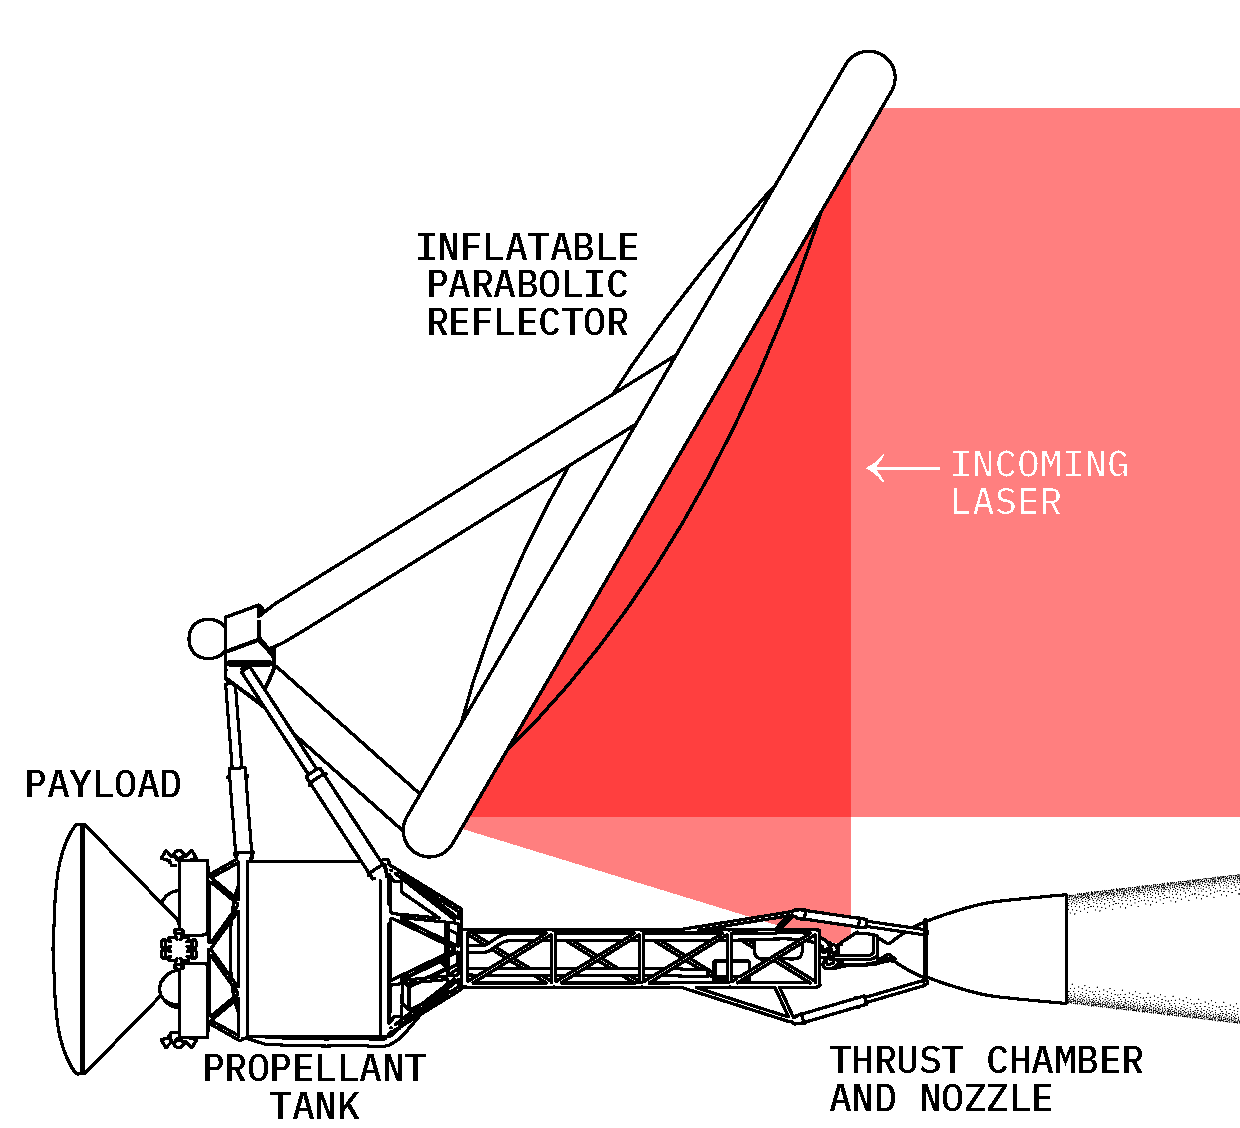
\includegraphics[width=\textwidth]{assets/2 background/overview_ltp}
                \caption{Spacecraft}
                \label{fig:overview_spacecraft}
            \end{subfigure}
            \begin{subfigure}[t]{0.64\textwidth}
                \centering
                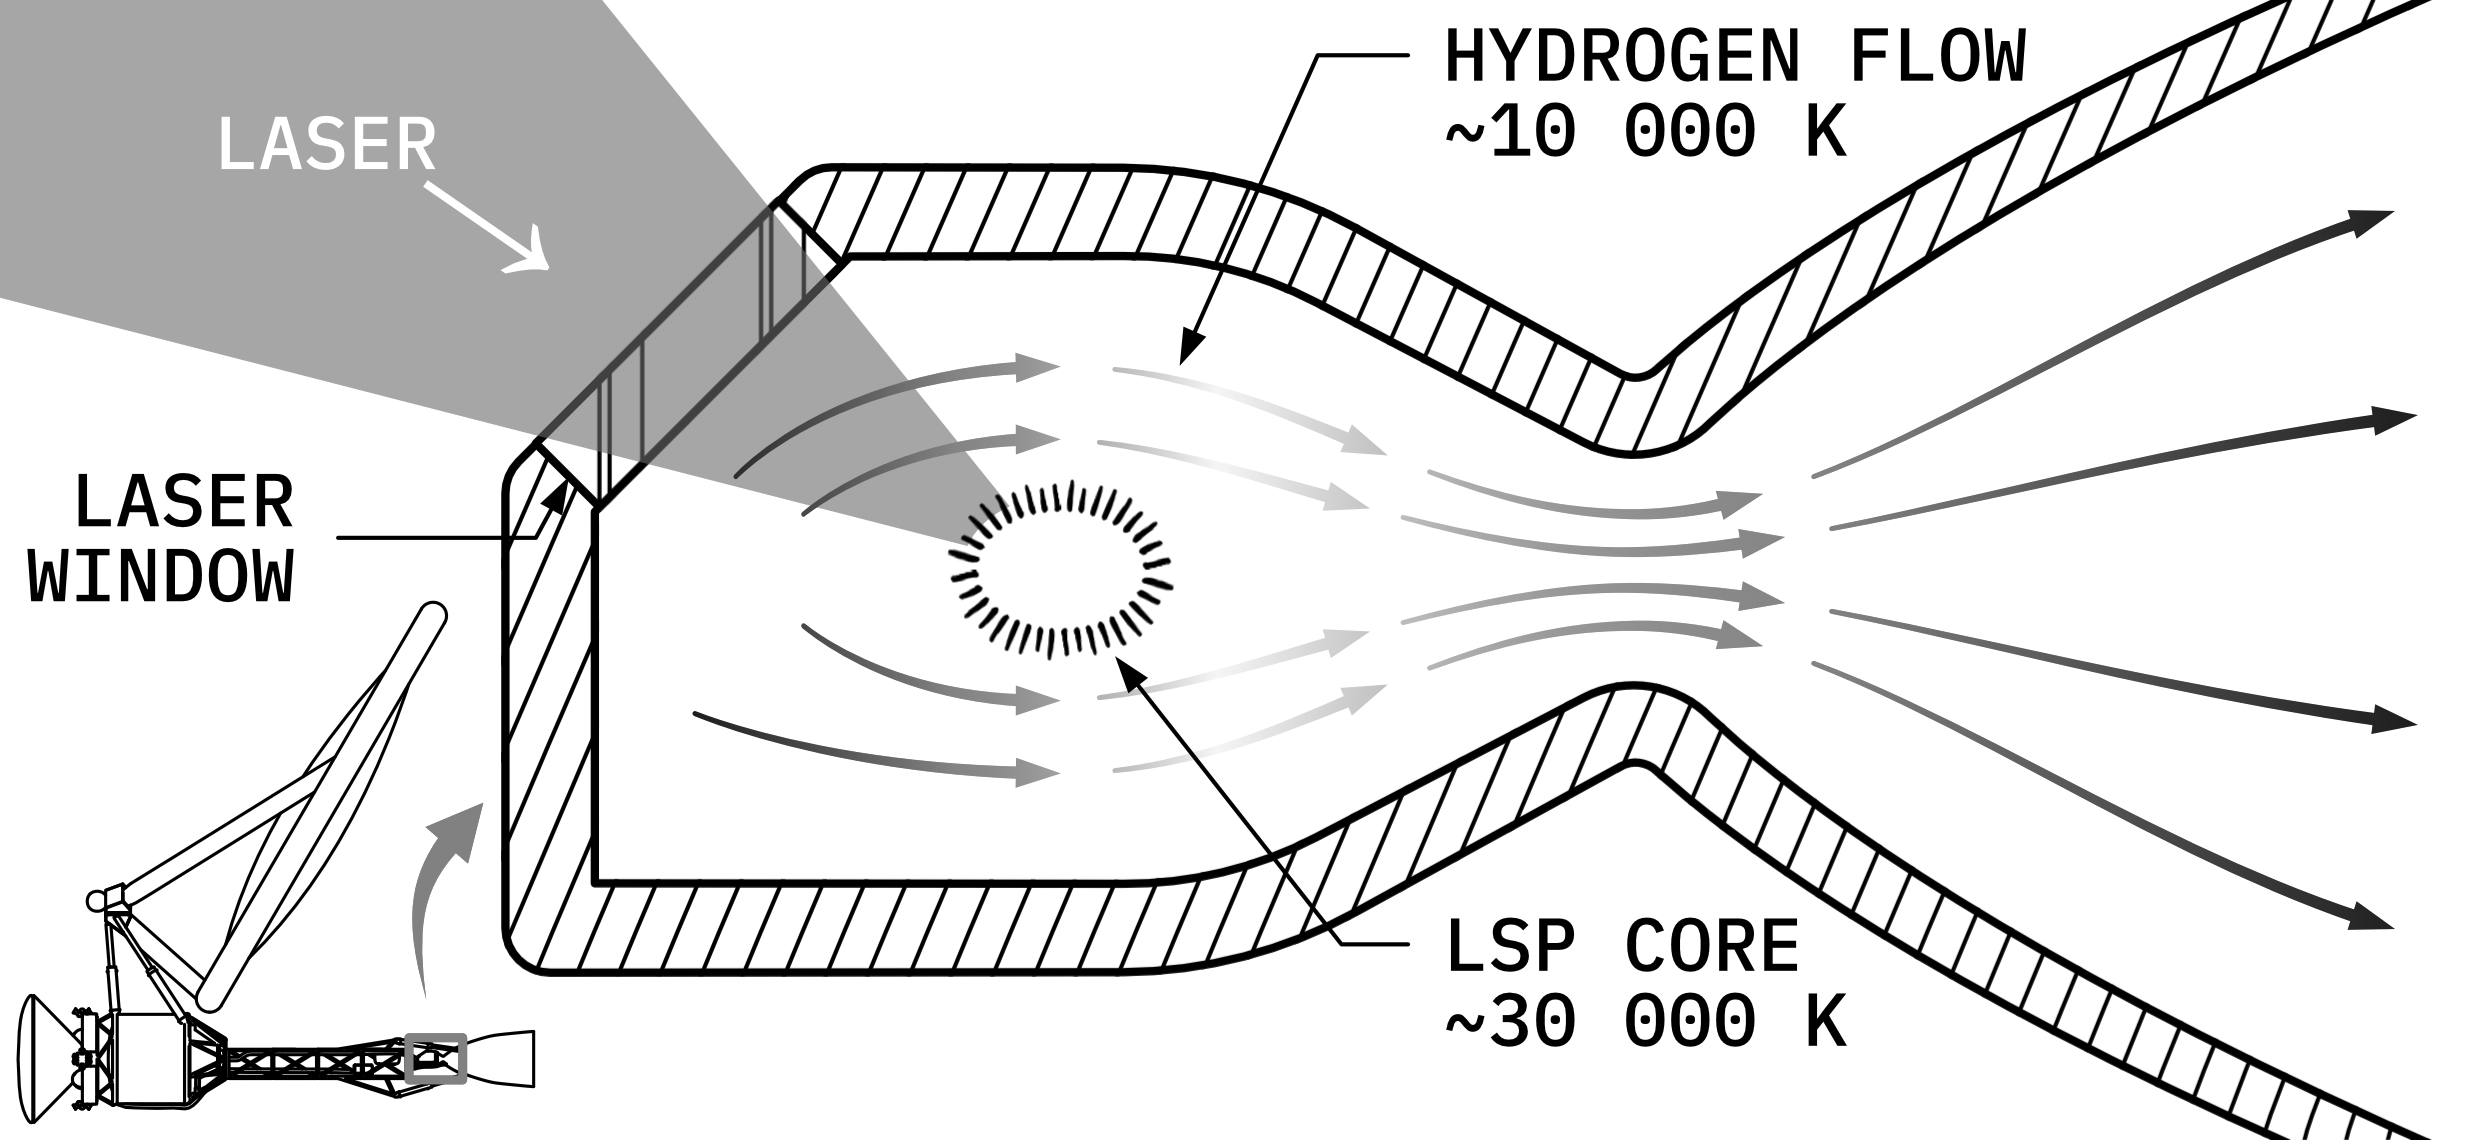
\includegraphics[width=\textwidth]{assets/2 background/chamber}
                \caption{Thrust chamber}
                \label{fig:overview_chamber}
            \end{subfigure}
            \caption[Overview of a CW laser-plasma LTP system]{Overview of a CW laser-plasma LTP system, adapted from \textcite{duplayDesignRapidTransit2022}}
            \label{fig:overview}
        \end{figure}

        As alluded to in the \nameref{chp:intro}, the key advantage of laser-thermal propulsion over chemical propulsion is its ability to deliver far greater exhaust velocities. Following from thermal rocket theory (\textcite{zandbergenAE4S01ThermalRocket2020}), the limiting exhaust velocity $v_\text{ex, max}$ of a thermal rocket motor depends on \autoref{eq:isp}, where $\gamma$ is the specific heat ratio of the propellant gas, $R_\text{u}$ is the universal gas constant, $\mathcal{M}$ is the propellant molar mass, and $T_\text{c}$ is the chamber temperature.
        \begin{equation}
            I_\text{sp, max}g_0 = v_\text{ex, max} \propto \sqrt{2\frac{\gamma}{\gamma-1}\frac{R_\text{u}}{\mathcal{M}}T_\text{c}} \label{eq:isp}
        \end{equation}
        All other parameters being equal, a thermal rocket engine operating at a higher chamber temperature will thus have a greater limiting exhaust velocity. By decoupling the thermal input from the propellant choice, unlike chemical thrusters whose chamber temperature is limited by their chemical reaction's adiabatic temperature, a laser-thermal rocket engine can readily attain temperatures of up to 10~000~K at the nozzle inlet, resulting in a specific impulse of more than 1000~s, as shown by \textcite{noredApplicationHighPower1976} in \autoref{fig:nored_Isp}.

        \begin{figure}[h]
            \centering
            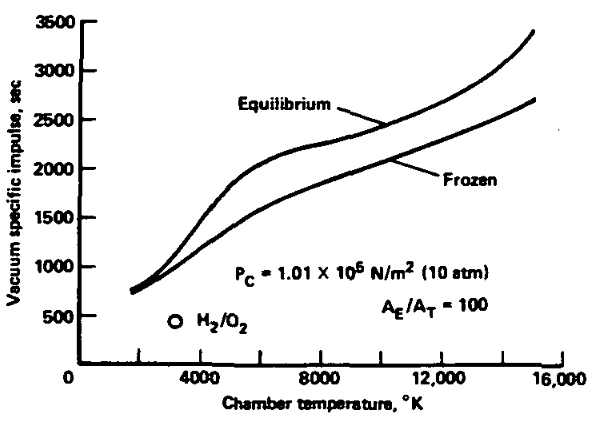
\includegraphics[width=0.7\textwidth]{assets/2 background/nored_ltpIsp.png}
            \caption[Theoretical specific impulse attained for a given hydrogen temperature]{Theoretical specific impulse attained for a given hydrogen temperature at the nozzle inlet, by \textcite{noredApplicationHighPower1976}. The specific impulse is bounded by two cases: 1.~the exhaust products maintain chemical equilibrium as they cool and expand through the nozzle; 2.~the composition of the exhaust is ``frozen''}
            \label{fig:nored_Isp}
        \end{figure}

        Some practical issues with this concept do remain. Although it is well understood that the high propellant temperatures that could be achieved by LTP would result in \qtyrange{1000}{3000}{s} of specific impulse (with hydrogen), whether or not the heat deposited in the LSP can be transferred to all the propellant flow with minimal losses is a critical issue. This problem was studied in-depth by \textcite{shojiPerformanceHeatTransfer1976}, who performed a thorough analysis of heat transfer within two LTP engines, proposing seeding the flow with carbon particles as a solution to reduce radiative heat losses to the chamber walls. Their analysis showed that such losses could be reduced to 4.5~\% of the input laser power, for hydrogen seeded with 50~\% carbon (by weight). While this is promising, such a system has yet to be tested experimentally. Furthermore, as suggested by \autoref{eq:isp}, the introduction of higher molar-mass carbon particles is associated with a penalty in the resulting specific impulse: \citeauthor{shojiPerformanceHeatTransfer1976}'s models show a decrease in theoretical specific impulse of around 25~\%.

        Cooling is also an issue. Even with the inclusion of carbon seeding, the magnitude of laser power considered for DEP (MW to GW) makes 4.5~\% of input power radiated to the thruster walls considerable. The propellant temperatures associated with high specific impulse are also far greater than the ones typically encountered by conventional thermal rocket engines, potentially necessitating new cooling strategies (\textcite{noredApplicationHighPower1976}). Thankfully, many of these cooling issues are similar in nature and magnitude to those encountered in Gas-Core Nuclear Rockets (GCNR), a sub-type of NTP. \textcite{kascakNozzleCavityWall1971} discusses a hydrogen GCNR operating at temperatures and specific impulses of the same order of magnitude, suggesting that a combination of transpiration cooling and gas seeding would be sufficient.

    \section{Laser-Sustained Plasma} \label{sec:background_lsp}
        One might wonder why bother with plasma at all. If the laser radiation could be deposited evenly in the propellant flow, little to no mixing would be needed and peak temperatures would be lower. Unfortunately, the use of lasers to directly heat hydrogen propellant has a major flaw: hydrogen gas does not absorb 1-\unit{\um}-wavelength radiation at room temperatures. Hydrogen only begins to absorb this wavelength at around 10~000~K, as shown by \textcite{glumbConceptsStatusLasersupported1984}: ``The paradox is that hydrogen cannot absorb any laser radiation unless it is already hot.'' They were considering 10.6 \unit{\um} laser radiation, but this also holds for 1.06 \unit{\um}. This is because these wavelengths do not match hydrogen's resonance absorption bands, whereby radiation is absorbed in the rotational or vibrational modes of a molecule. The main absorption mechanism in LSP is \emph{inverse bremsstrahlung} (IB): free electrons absorb radiation across a continuous spectrum (as opposed to specific wavelengths) during collisions with ions in the plasma (\textcite{keeferLaserSustainedPlasmas1989}). \textcite{johnstonCorrectValuesHighfrequency1973} showed that the radiation absorption coefficient $\alpha$ [\unit{m^{-1}}] can be calculated with \autoref{eq:ib_absorption}, where $Z$ is the ionic charge state (=1 for single-ionization), $n_\mathrm{e}$ is the electron density, $\nu$ is the radiation frequency, $k_\mathrm{B}$ is the Boltzmann constant, and $T_\mathrm{e}$ is the electron temperature in Kelvin. The Coulomb logarithm $\ln{\Lambda}$ and the plasma frequency $\nu_\mathrm{p}$ will be discussed in further detail in \autoref{chp:models}.
        \newcommand{\ibalphaeq}{\alpha = \frac{7.8\times 10^{-7}Zn_\mathrm{e}^2\ln{\Lambda}}{\nu^2(k_\mathrm{B}T_\mathrm{e})^{3/2}} \left(1-\frac{\nu_\mathrm{p}^2}{\nu^2}\right)^{-1/2}}
        \begin{equation}
            \ibalphaeq \label{eq:ib_absorption}
        \end{equation}

    \section{Past experiments} \label{sec:background_exp}

    \section{Research objectives}